\documentclass[conference]{IEEEtran}
\IEEEoverridecommandlockouts
% The preceding line is only needed to identify funding in the first footnote. If that is unneeded, please comment it out.
\usepackage{cite}
\usepackage{amsmath,amssymb,amsfonts}
\usepackage{algorithmic}
\usepackage{graphicx}
\usepackage{textcomp}
\usepackage{xcolor}
\def\BibTeX{{\rm B\kern-.05em{\sc i\kern-.025em b}\kern-.08em
    T\kern-.1667em\lower.7ex\hbox{E}\kern-.125emX}}
\begin{document}

\title{Addressing Crash Recovery With Persistent Memory Allocation\\
{\footnotesize \textsuperscript{}}
}

\author{\IEEEauthorblockN{\textsuperscript{} Nicholas Stone}
\IEEEauthorblockA{\textit{Xavier University} \\
Cincinnati Ohio, USA \\
Stonen2@Xavier.edu}
\and
\IEEEauthorblockN{\textsuperscript{} Michael Spear}
\IEEEauthorblockA{\textit{Lehigh University} \\
\textit{Bethlehem Pennsylvania, USA}\\
spear@lehigh.edu}
\and
\IEEEauthorblockN{\textsuperscript{} Roberto Palmieri}
\IEEEauthorblockA{\textit{Lehigh University} \\
\textit{Bethlehem Pennsylvania, USA}\\
palmieri@lehigh.edu}
}
\maketitle

\begin{abstract}
Persistent memory is a combination of both volatile memory and long-term storage.  This means Persistent memory is able to maintain the speed of volatile memory such as Dynamic Random-Access Memory (DRAM) and is like the long-term storage of devices such as Solid-State Drive (SSD) and Hard Disk Drive (HDD), in its ability to maintain its state without consuming power. Furthermore, since persistent memory has Byte addressability and long-term storage, allocators can be used to maintain Data-structures that will persist even after power failure or program crashes. While persistent memory has unique characteristics that DRAM does not have, persistent memory has a few draw backs. Excessive writes to a single memory cell can destroy it and writes on persistent memory are much slower than reads. In this project we will be creating a memory allocator that will leverage both DRAM and Non-Volatile Random-Access Memory (NVRAM) to perform smart memory allocation that will be able to allow a data structure’s integrity to be preserved despite crashes and power failures without excessive writing to the persistent memory.
\end{abstract}

\begin{IEEEkeywords}
HDD,SSD,allocator,NVRAM,Persistent Memory
\end{IEEEkeywords}

\section{Introduction}
Non-Volatile Random-Access Memory (NVRAM) is a new kind of persistent memory that has a few unique characteristics that are different than that of Random-Access Memory (RAM).  The first is that this new form of technology allows for byte addressable long-term storage means that operate and execute several orders of magnitude faster than that of both Hard Disk Drives (HDD) and Solid-State Drives (SSD). Another unique factor of NVRAM is that this form of technology has a limited number of writes before the memory cells becomes unusable. If a program is not implemented properly or poorly the program can destroy memory cells rapidly thus damaging the technology and rendering it more expensive to use than typical RAM. One of the underlying tools that a programmer does not need to worry about usually is the allocator that a program is running or using.  Meaning that if a programmer was to write a program that was constantly writing to the same memory cells this could lead to a short life span of the NVRAM technology. It then becomes critical the smart memory allocations and tactical memory writes is used to leverage the NVRAM technology to be most effective. 
Memory allocators have been used in systems since the early 1960s with the buddy memory allocation being implemented and used in 1963. As described above NVRAM has some unique properties that will enhance the runtime and performance of programs. However, if the same memory allocators that are used for RAM are used for NVRAM a large performance increase might not be experienced since these tactics are designed to run efficiently on RAM. The Memory allocating tactics that are used in this paper and program inherit some of the same or similar tactics to those that run on RAM but have a few unique characteristics that make them different. The first is that while locality is important for RAM technologies locality is critical for NVRAM technologies. Since NVRAM allows for data to persist even when a power cycle happens this means that any data in memory will be preserved on start up. Thus, allowing for a second program or an allocator to go through and find and restore all data that a program would have been using before a power cycle.  If a program can execute a systematic approach to memory allocation, then a simple algorithm can be implemented to then restore data in a quick and efficient manner. The second thing is that custom memory allocators may become more beneficial on NVRAM technologies than that of RAM. This is due to the fact that NVRAM could be leveraged in a variety of ways by many different systems, meaning that a DMBS might use NVRAM to hold ‘Hot’ Tuples while a Cloud system might use allocation tactics differently.  The following memory allocator aims to see what kind of allocation tactics yields the best performance for programs while utilizing both RAM and NVRAM technologies. 


\section{Background}
The following section will explain the two main components that this paper focuses on, NVRAM and memory allocation. The following will not go into detail about the algorithms or tactics that the memory allocation in this paper will use, those details will be explained in further detail later on in this paper. 
\subsection{Persistent Memory Non-Volatile Random Access Memory}
NVRAM is a new and emerging kind of persistent memory that acts very similarly to RAM but also has a few key differences. The major differences are that this form of memory allows for byte addressability and has a much faster write time than that of both Hard Disk Drives (HDD) and Solid-State Drives (SSD). This order of magnitude is also followed by similar read times as that of RAM. Continuing from this NVRAM has the ability for data being stored to have long term storage like that of HDD or SSD when a power cycle occurs. One of the main drawbacks of NVRAM is that the memory has a write endurance, meaning that if too many write occur in a given memory cell that memory cell can be destroyed and no longer used. Obviously when memory cells are destroyed more writes will occur over more memory cells causing the destruction of NVRAM to happen quickly. NVRAM is not going to be replacing RAM in this allocation tactic but will be used alongside RAM. By leveraging both technologies we hope to allow preservation of data as well as long term use of the NVRAM technology.
\subsection{Memory Allocation}
A memory allocator is a program that is responsible for maintaining and distributing memory to be used by other programs. Part of the maintaining process is to make sure that all memory is distributed with the goal of locality as well as making sure that memory is returned to the operating system once the program no longer needs it. In this paper the main memory allocation tactic used is arena allocation, or the method of sectioning off large chunks of memory and then further distributing smaller sections of memory to be used by a program. By using this type of allocation, a second level of abstraction is added to the memory allocation and allows for arenas to maintain already allocated sections of memory while the allocator is able to distribute more arenas to a program. This allows for concurrency to flow in a program and can help stop bottle necks from occurring. This form of dynamic memory allocation is only one of many and used arenas in all of the data structures that will be listed here after. 


\section{Related Work}
\subsection{HOARD}
\subsection{MAKALU}
\subsection {REWIND} 

\section{Problems}
As mentioned above the NVRAM has both pros and cons and while the pros can be used to increase performance in programs the cons can lead to devastating impacts in the long term for a program. For example, if the creation of an allocator that only leverages NVRAM technologies might have an immediate increase in runtimes the lifetime of the NVRAM will be minimal as well as current RAM allocating tactics will not utilize NVRAM to is full potential. New allocating tactics should be examined since locality of memory in for NVRAM is critical as well as using both RAM and NVRAM in order to make a reliable and fast allocator becomes the main goal. The biggest problem then becomes understanding which of the many allocating tactics would be most efficient on this new technology. 
\section{Implementation Problems}
Before undertaking this project, I had done minimal systems work and even less work pertaining to memory allocators and changing the way that memory is allocated in a program beyond New and delete. The first of the many implementation problems that occurred was understanding the data structures and how they work together to achieve an efficient means to allocate memory. The implementation problem then occurred with linking the idea of an arena and how each arena needs to store a data structure or bit map to be able to track which parts of the memory have been allocated. The next implementation obstacle was building data structures and the level of abstraction for arena’s that allow for strong locality. Meaning that all of the data is being stored in or near one another. The last implementation problem that I will highlight in this paper is understanding which memory preservation tactic would work best and most efficient at the same time. With the instruction of placement new it became difficult to write reliable algorithms using placement new without overwriting nodes that are still in use.  
\section{Implementation Solutions}
In systems the greatest implementation solution that I have found to help solve all of my problems is to start with a picture. Meaning that when implementation problems occurred such as not fully understanding how the bitmap would interact with the arena data structures once a picture was drawn further ideas and tactics could be understood and then implemented. Not all of the ideas that are gathered from a picture work or are efficient, but it was a clear way of understanding the data structures. As for allocation tactics that would be used to reclaim memory with instructions such as placement new the tactic of free was to be changed to understand how much the free function will impact performance. Namely this meaning that free would not free any memory back to the OS but would reset an arena back to be completely cleared of all data and was ready to be used by the program. 
\section{Visualization of Data-Structure} 
As discussed previously in this paper the goal of the NVRAM allocator is to make sure that locality is key, or the goal is making sure all data structures are placed in memory in some form of sequential chain. This allows a program to very quickly traverse the data structures and then allocate memory to the programmer. Here after will show the transformation in the data structure and show the improvement in locality as well as use of the free list algorithm. 
\subsection{Iteration 1}
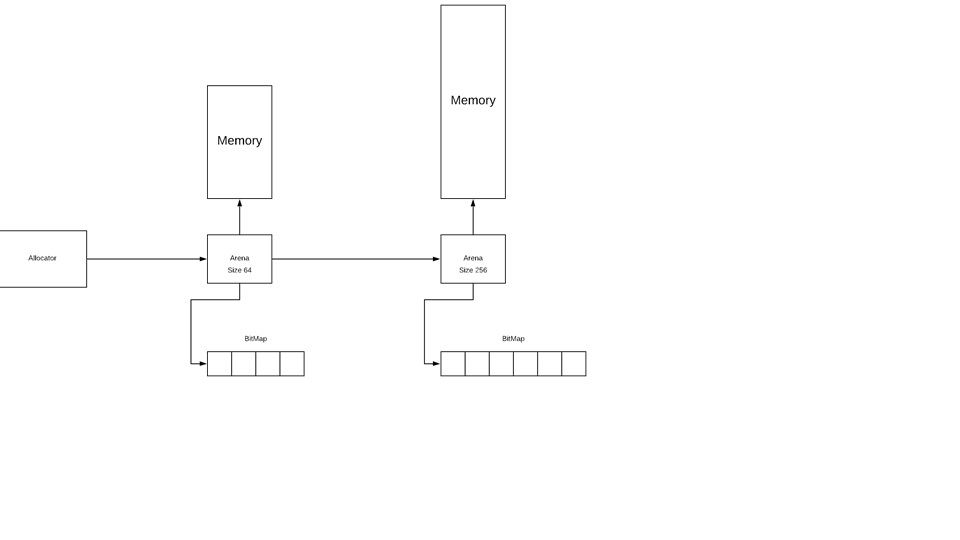
\includegraphics[width=14cm]{iteration1datastructure.jpg}
\caption{First Iteration of the Arena Data Structure}
\label{fig1:Iteration1}
\\


\subsection{Iteration 2} 
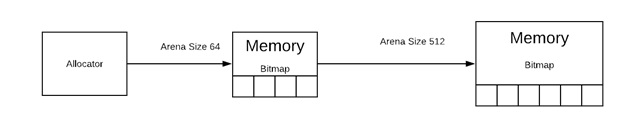
\includegraphics[width=8cm]{Iteration2datastructure.jpg}
\caption{Second Iteration of the Arena Data Structure}
\label{fig2:Iteration2}

\subsection{Iteration 3}
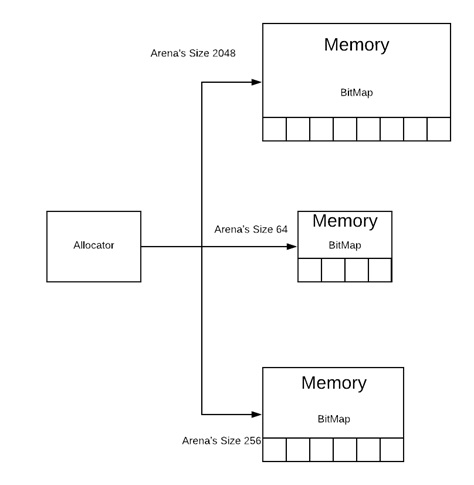
\includegraphics[width=8cm]{Iteration3datastructure.jpg}
\caption{Third Iteration of the Arena Data Structure}
\label{fig3:Iteration3}



\section{Evaluation}
Place Holder

\section{Future Work}
The project currently provides a strong base and API that replicates and allows programmers to use an allocator that implements a form of smart allocating tactics. However, since NVRAM is a relatively new form of technology there are very few other kinds of NVRAM aware allocators. Thus, it would be unfair to compare speeds of NVRAM technologies against RAM technologies since as described above the technologies are different. From this future work on this project and allocator Is to implement at least two other kinds of allocators and compare these speeds against one another as well as RAM technologies. Along with these implementations the need for investigation in which concurrency tactic should be implemented. While ideally atomic operations should be utilized experiments of other kinds of concurrency tactics should be used in order to give programmers ideas of which method would be best for implementation of custom allocators. Mainly the goal of this second part is to share information of is the performance increase of atomic operations worth the time it takes to implement atomic allocations versus that of a spin lock allocation tactic. 

\section{Future Experiments}
It is important that experiments for all of the allocators that are tested, are executed on the basis of not only runtime performance but as well as concurrency and crash recovery. Namely that allocation times such as malloc and free should be tested but also the amount of time that each thread takes as well as the overall recovery time needs to be examined. That is if an arena allocator has poor free time, but recovery time is much faster that that of another form of dynamic memory allocation then use cases need to be examined before one type of allocator can be favored on NVRAM. Furthermore, the investigation of allocator data structures should also be examined, allowing a programmer to identify which type of data structure allows for fastest runtime. This means examining a free list tactic versus best fit tactic or a combination of both. 

\section{Conclusion}


\section{Acknowledgment}

The preferred spelling of the word ``acknowledgment'' in America is without 
an ``e'' after the ``g''. Avoid the stilted expression ``one of us (R. B. 
G.) thanks $\ldots$''. Instead, try ``R. B. G. thanks$\ldots$''. Put sponsor 
acknowledgments in the unnumbered footnote on the first page.

\section{References}

Please number citations consecutively within brackets \cite{IEEEhowto:IEEEtranpage}. The 
sentence punctuation follows the bracket \cite{b2}. Refer simply to the reference 
number, as in \cite{b3}---do not use ``Ref. \cite{b3}'' or ``reference \cite{b3}'' except at 
the beginning of a sentence: ``Reference \cite{b3} was the first $\ldots$''

Number footnotes separately in superscripts. Place the actual footnote at 
the bottom of the column in which it was cited. Do not put footnotes in the 
abstract or reference list. Use letters for table footnotes.

Unless there are six authors or more give all authors' names; do not use 
``et al.''. Papers that have not been published, even if they have been 
submitted for publication, should be cited as ``unpublished'' \cite{b4}. Papers 
that have been accepted for publication should be cited as ``in press'' \cite{b5}. 
Capitalize only the first word in a paper title, except for proper nouns and 
element symbols.

For papers published in translation journals, please give the English 
citation first, followed by the original foreign-language citation \cite{b6}.

\bibliographystyle{./bibliography/IEEEtran}
\bibliography{./bibliography/IEEEabrv,./bibliography/IEEEexample}

\vspace{12pt}
\color{red}
IEEE conference templates contain guidance text for composing and formatting conference papers. Please ensure that all template text is removed from your conference paper prior to submission to the conference. Failure to remove the template text from your paper may result in your paper not being published.

https://people.cs.umass.edu/~emery/pubs/berger-oopsla2002.pdf

https://people.cs.umass.edu/~emery/pubs/berger-oopsla2002.pdf

http://www.vldb.org/pvldb/vol8/p497-chatzistergiou.pdf

https://link.springer.com/chapter/10.1007/978-3-662-53426-7_23

https://dl.acm.org/citation.cfm?id=3054780

https://dl.acm.org/citation.cfm?id=2984019




\end{document}

